\section{Arhitectura aplicației} \label{arhitectura}
    \noindent Aplicația conține un audio plugin exportat în format VST3, AU și Standalone scrisă în C++ folosind JUCE, un modul scris în python pentru generarea secvențelor muzicale, precum și o librărie comună scrisă în C++ folosind Pybind11. 
    \begin{figure}[H]
        \centering
        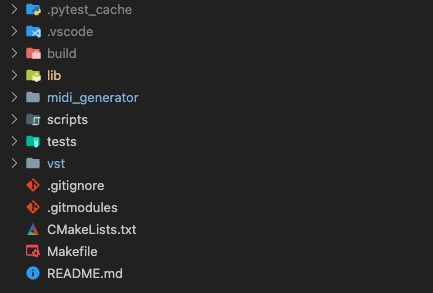
\includegraphics[scale=0.6]{images/structura.jpeg}
        \caption{Structura proiectului după build}
        \label{fig:structure}
    \end{figure}
    
    \subsection{Structură}
        \noindent Aplicația e construită folosind cmake și make, și a fost testată pe Debian 11 ARM și macOS 12. Pentru a putea utiliza aplicația, următoarele dependențe trebuiesc instalate:
        \begin{itemize}
            \item Python 3.10 (versiunea dev)
            \item CMake 3.23
            \item Make 4.3
            \item Clang 11
        \end{itemize}
        
    \subsection{Librării}
        \noindent \textbf{Boost} \par
        \noindent Boost este o colecție de librării scrise în C++ care implementează funcționalități folosite frecvent în dezvoltarea software. Dintre acestea, am folosit librăriile de logging și cel de testare unitară. \par 
        \noindent \textbf{Pybind11} \par
        \noindent Pybind11 este o librărie care permite interoperabilitate între C++ și python. Aceasta este folosită în aplicație pentru a facilita crearea unei interfețe de comunicare între plugin și modulul genetic. Un exemplu conținând implementarea endpoint-ului pentru apelarea funcției de generare din cadrul algoritmului genetic se poate găsi în Anexa \ref{Boost}. \par
    
    \subsection{Build tools}
        \noindent \textbf{Make} \par
            \noindent Pentru construirea, testarea și depanarea aplicației am folosit Make și CMake. În Make sunt definite 7 sarcini executabile:
            \begin{itemize}
                \item \textbf{config} - configurează structura proiectelor CMake.
                \item \textbf{build-lib} - construiește librăria comună folosită de plugin si modul.
                \item \textbf{build} - construiește modulul de python și pluginul standalone.
                \item \textbf{test} - execută testele unitare conținute în aplicație.
                \item \textbf{run} - rulează pluginul standalone.
                \item \textbf{clean} - șterge folder-ul în care este construită aplicația (build) și fișierele temporare create de python.
                \item \textbf{all} - execută în ordinea config\rightarrow build-plugin\rightarrow build\rightarrow test\rightarrow run.
            \end{itemize}
        \noindent \textbf{Cmake} \par
            \noindent CMake este unealta de împachetare principală folosită. Aplicația folosește 4 fișiere de configurare pentru crearea executabilului final. Primul dintre acestea este conținute în directorul principal al aplicației și reprezintă punctul de început al configurație (Anexa \ref{CMake}). Aici sunt căutate librăriile din python și boost și executabilul de python și sunt incluse în configurație, după care este configurată librăria comună și este construit și instalat modulul genetic. Apoi, sunt adăugate și configurate modulele folosite în cadrul plugin-ului, urmate de plugin-ul audio și configurarea testelor. \par
            Următorul fișier de configurare este localizat în directorul în care este conținută librăria comună și are scopul de a o construi și adăuga în configurație. Directorul în care se crează plugin-ul audio conține de asemenea un fișier de configurare, care crează executabilele în format .VST, .AU și Stanadalone, și include modulele folosite. Ultimul fișier este localizat în directorul care conține testele unitare și este folosit pentru a crea mai multe executabile, reprezentând suite de teste.
        
    \subsection{Testare}
        \noindent Aplicația conține teste unitare scrise folosind pytest (pentru testarea modulului) și librăria de teste unitare conținute în boost (pentru librărie comună și plugin-ul audio). Acestea sunt folosite în special pentru a verifica daca este configurată corect comunicarea între componentele distincte ale aplicației. 
        \par Un exemplu de suită de teste este inclusă în anexa \ref{Testare}, folosit pentru a verifica dacă librăria poate traduce informație legată de notele muzicale din Python în C++ și invers. Celelalte suite de teste verifică dacă librăria dinamică este încarcată corect la runtime, funcționarea corespunzătoare a API-ului și funcționarea comenzilor conținute în modulul genetic.
 